\documentclass[a4paper,11pt]{article} 

% \documentclass[a4paper,11pt]{book} 

\usepackage[T1]{fontenc}
\usepackage[utf8]{inputenc}
\usepackage[spanish]{babel}

\usepackage{graphicx}

\usepackage{colortbl}
\usepackage{color}

\usepackage{hyperref}

\usepackage[margin=1in]{geometry}
\pagestyle{plain}

%\usepackage{fancyhdr} 
%\usepackage{lastpage}
%\usepackage{float} 
%\floatstyle{boxed} 
%\restylefloat{figure} 
%\pagestyle{fancy}

\setcounter{secnumdepth}{5}
\setcounter{tocdepth}{6}

\definecolor{orange}{RGB}{0,0,255}
\setcounter{secnumdepth}{5}
\setcounter{tocdepth}{5}
%\title{\textcolor{orange}{Guia Practica Instalación de MinSoc}}
%\author{Gomez,Roberto Pablo - Lovaisa Michelini, Valeria  \\ Universidad Tecnológica Nacional \\ CUDAR }

\begin{document}

%\lhead{\includegraphics[width=1\textwidth]{encab.png}}
%\lfoot{{\includegraphics[width=1\textwidth]{pie.png}}}
%\rfoot{\thepage}

%\maketitle 
%\newpage

\tableofcontents


\newpage

\section{\textcolor{orange}{Introducción}}
\subsection{\textcolor{orange}{Descripción General}}
Descripción por arriba del trabajo. por ejemplo la industria dispone de herramientas que nosotros usamos para un fin determinado.

\subsection{\textcolor{orange}{Objetivos}}
\subsubsection{\textcolor{orange}{Objetivo General}}

Implementar un system on chip OpenSource con un microprocesador embebido Soft-core que soporte un sistema operativo libre , con la finalidad de entregar un sitema integral FPGA-SoC-Sistema Operativo completamente funcional y bajo licencia GPL v2.

\subsubsection{\textcolor{orange}{Objetivo Específico}}
\begin{itemize}
\item Seleccionar, analizar y determinar un microprocesador Sof-Core.
\item Establecer un system on chip Open Source donde poder implementar un Soft-Core.
\item Determinar sistemas operativo con licencia GPL v2 que tengan las prestaciones funcionales adecuadas.
%\item Evaluar, seleccionar una plataforma objetivo un entorno de trabajo  las prestaciones de los Kit de desarrollos con FPGA disponibles en el área de trabajo.
%\item Evaluar, seleccionar y validar las prestaciones de los Kit de desarrollos con FPGA disponibles en el área de trabajo.
%\item Analizar un soft-core que me de las prestaciones funcionales que cumplan de  los requerimientos 
%\ Obtener  completamente funcional sobre un kit de desarrollo XILINX XtremeDSP Starter Platform Spartan 3A DSP 1800.
%\item Implementar un Sistema Operativo eCos sobre un SoC de codigo abierto en el Kit de desarrollo XILINX XtremeDSP Starter Platform Spartan 3A DSP 1800.
%\item Implementar un Sistema Operativo Linux sobre un SoC de codigo abierto en el Kit de desarrollo XILINX XtremeDSP Starter Platform Spartan 3A DSP 1800 .
%\item Probar el adecuado funcionamiento de el sistema global que tenga las  prestaciones funcional  
%tradicionales de diseño
\end{itemize}

\subsection{\textcolor{orange}{Motivación}}

Existe un grupo de cores Sof-Core de código abierto que no están limitados por la tecnología. Los cores destacados de microprocesadores de 32 bits, son los procesadores SPARC LEON OpenRISC 1200 , y el core de LatticeMico32. Usar cores de  codigo abierto,  va unido a una serie de conceptos como:
 \begin {itemize}
\item Flexibilidad. Si el codigo fuente está disponible, los desarrolladores pueden modificar el codigo de acuerdo a sus necesidades.Adémas, se produce un flujo constante de ideas que mejora la calidad del codigo.
\item Fiabilidad y seguridad. Con muchos programadores a la vez escrutando el mismo trabajo, los errores se detectan y corrigen antes, por lo que el producto resultante es mas fiable y eficaz que el comercial.
\item Rapidez de desarrollo. Las actualizaciones y ajustes se realizan a través de una comunicación constante vía Internet.
\item Relación con el usuario. El programador se acerca mucho mas a las necesidades reales de su cliente, y puede crear un producto especifíco para él
 \end {itemize}
 
Obtener un sistema integral de código abierto en donde se tiene código HDL, assembler y C disponible para adaptarse de acuerdo a los requerimientos del proyecto. Ademas de la de la capacidad de migrar de una plataforma a otra. Logrando menor dependencia entre el código fuente y la plataforma objetivo. 
La portabilidad del codigo abierto nos permite implementarlo sobre una ASICs (Application-specific integrated circuit) o con modificaciones menores en cualquier FPGA (Field Programmable Gate Array) de Xilinx, Altera, Lattice, etc. 

Estos tres de los más grandes proveedores de FPGA , Xilinx , Altera y Lattice , ofrecen sus propios micro core RISC de 32bits los dos mayores proveedores de dispositivos FPGA , Altera y Xilinx , proporcionan el micro core Nios y Microblaze, respectivamente. Son micro cores  en donde el codigo fuente RTL no se encuera disponible y solo pueden ser implementados en sus respectivas FPGA.
 
Una de principales ventajas de usar plataformas con FPGA, es que son flexibles asi que pueden adaptarse a diferentes funciones. Los componentes de hardware ofrecen mucho mayor rendimiento que el software equivalente. Los cuellos de botella de procesamiento del sistema pueden identificarse y sustituirse por hardware, de manera que se evita la costosa optimizan del software.

\subsection{\textcolor{orange}{Importancia del Problema}}

En el diseño del sistema embebido se usan diferentes procesos depende del tipo de sistema, el hardware disponible y la organización que desarrolle el sistema. Una de las actividades principales en un proceso de diseño de software es la elección del hardware y del sistema operativo que se efectúa antes del comienzo del software. Ante tal situación , se debe diseñar el software par considerar las restricciones impuestas por las capacidades del hardware.
Los efectos que influyen dichas elecciones comprenden restricciones de de temporización sobre el sistema, limitación en la energía disponible, experiencia del equipo de desarrollo y limites en el costos del sistema entregable.
 
Se está explorando una linea donde se busca dar al diseñador del sistema embebido una solución flexible en la primera etapa de la elección de plataforma. Donde a través del análisis de diferentes plataformas de desarrollo OpenSource y privativas pueda elegir la mejor opción para el tipo de sistema a desarrollar y requerimientos de proceso. 
 
Una vez que se ha elegido la plataforma de ejecucion para el sistema, se ha diseñado una arquitectura de proceso y se a determinado una políticas de planeación, es necesario comprobar que el sistema cumplirá sus con sus requerimientos.

\subsection{\textcolor{orange}{Alcance del Estudio}}

Debido al plazo estipulado para el desarrollo del proyecto, el mismo involucra tres etapas: 

 \begin {itemize}
\item Especificación y Análisis de requerimientos.
\item Implementación.
\item Testing.
 \end {itemize}


%de donde hasta donde vamos a ir
%primero elegimos un micro después lo embebemos en un soc y después le metimos un sistema operativo
\subsection{\textcolor{orange}{Modelo de Desarrollo}}


El modelo de desarrollo a utilizar es el Modelo en Espiral tipificado por Ian Sommerville [2] . El modelo en espiral de ingeniería de software, mostrado en la Ilustración 1, fue originalmente propuesto por Boehm en año 1988, en su artículo A Spiral Model of Software Development and Enhancement. Propuso un marco del proceso de software dirigido por el riesgo. Aquí, el proceso de software se representa como una es espiral, cada ciclo en la espiral representa una fase del proceso de software. Por ende el, ciclo más interno puede relacionarse con la factibilidad del sistema, el siguiente ciclo con la definición de requerimientos, el siguiente ciclo al diseño del sistema, y así sucesivamente.
Cada ciclo del espiral se divide en 4 sectores:
 
\begin {itemize}
\item Establecimiento de objetivo  Se definen objetivos específicos para dicha fase del proyecto. Se identifican restricciones en el proceso y el producto, y se traza un plan detallado de gestión. Se identifican los riesgos del proyecto. Dependiendo de estos riegos, se planean estrategias alternativas
\item Validación y reducción del riesgo  En cada uno de los riesgos identificados del proyecto, se realiza un análisis minucioso. Se dan acciones para reducir el riesgo.
\item Desarrollo y validación  Despues de una evaluacion del riesgo, se elige un modelo de desarrollo para el sistema.
\item Planeción  El proyecto se revisa y se toma una decisión sobre si hay que continuar con otro ciclo de la espiral. Si se opta por continuar, se trazan los planes para la siguente fase del proyecto.
 \end {itemize}mn

Como característica principal de esta metodología es que posee una consideración explícita del riesgo. Informalmente, el riesgo significa sencillamente que algo puede ir mal. Los riegos originan problemas en el proyecto, como los de confección de agendas y excesos en los costos; por lo tanto, la disminución de riegos es una actividad sumamente importante en la gestión del proyecto.
Un ciclo en la espiral comienza con la elaboración de objetivos, como el rendimiento y la funcionalidad. Entonces se enumeran formas alternativas de alcanzar estos objetivos y las restricciones impuestas en cada una de ellas. Cada alternativa se evalúa contra cada objetivo y se identifican las fuentes de riegos del proyecto. El siguiente paso es resolver estos riesgos mediante actividades de recopilación de información como la de detallar más el análisis, la construcción de prototipos y la simulación. Una vez que se han evaluado los riesgos se llevará a cabo cierto desarrollo, seguido de una actividad de planificación para la siguiente fase del proceso.

\subsection{\textcolor{orange}{Metodología}}

Considerando que el objetivo planteado es un desarrollo que se realiza por primera vez, se aplicará un desarrollo experimental y de simulación. La falta de documentación al respecto y al ser un desarrollo de vanguardia son factores que acentúan en esta decisión. Sumado a lo anteriormente dicho, en el laboratorio donde se desarrolla este proyecto no existen antecedentes de trabajos similares.
 
Se utilizó como metodología en este desarrollo el modelo de componentes, donde se define estándares para la implementación, documentación y el despliegue de componentes. 


%\section{\textcolor{orange}{Perspectiva Historica}}
%	\subsection{\textcolor{orange}{El Comienzo de los Microprocesadores}}
%	\subsection{\textcolor{orange}{FPGAs y Microsprocesadores Soft-Core}}
%	\subsection{\textcolor{orange}{Software OpenSource y Libre}}
 %%%%%%%%%%%%%%%%%%%%%%%%%%%%%%%%%%%%%%%%%%%%%%%%%%CAPITULO 2%%%%%%%%%%%%%%%%%%%%%%%%%%%%%%%%%%%%%%%%%%%%%%%%%%%%%%%%%%%%%%%%

\section{\textcolor{orange}{FPGA y microprocesadores Soft-Core}}%julius
	\subsection{\textcolor{orange}{FPGAs}}

La fabricación de dispositivos semiconductores es un proceso complicado de plazos largos y costoso. Esto lleva a que los diseños destinados para la  implementacion en chip de silicio tengan poco oportunidad de ser prototipados antes de que comience la producción en grandes volúmenes. Esto supone una gran importancia  en las faces de prueba y verificación de un diseño antes de ser fabricado.

Basándose en la predicción de la ley de Moore donde expresa que aproximadamente cada dos años se duplica el número de transistores en un circuito integrado\cite{Etiqueta01}, Ross Freeman postulo que los transistores serian menos costoso cada año, haciendo asequible la fabricación de chips programables personalizables \cite{Etiqueta03}.
La compañía Xilinx, ofreció su primer chip en 1984 , que contiene arrays celdas lógicas (LCAs) , programables por el usuario en casi cualquier configuración que quisieran. Estos se conocen como Field Programmable Gate Array (FPGAs) .

Las FPGAs desempeñan un papel dual, uno como objetivo final de ejecución en un diseño y otro papel como prototipo para la implmentacion definitiva de un diseño. Su capacidad de reconfigurar el diseño parcial o totalmente para su actualización o corrección de errores tiene un costo relativamente bajo a diferencia del prototipado sobre ASICs.
Actualmente las FPGA cuentan con una gran cantidad de recursos disponibles (Compuertas lógicas , Bloques de RAM) para implementar diseños digitales complejos.

Una desventaja de las FPGA  es debido a la naturaleza inherente de las arquitecturas de FPGA, los diseños implementados en FPGA comparados con una ASICs en general tienen mas area, menos porformance y consumen mas energía.

		\subsubsection{\textcolor{orange}{Arquitectura}}	

Los componentes de una \textit{FPGA} se pueden dividir en cinco grupos:

\begin {itemize}
\item  Bloques lógicos configurables y \textit{Lookup Tables}.
\item  Bloques de entrada y salida.
\item  Bloques multiplicadores
\item  Bloques Manejadores de Clock Digitales.
 \end {itemize}

\begin{figure}[h!]
 \begin{center}
 % 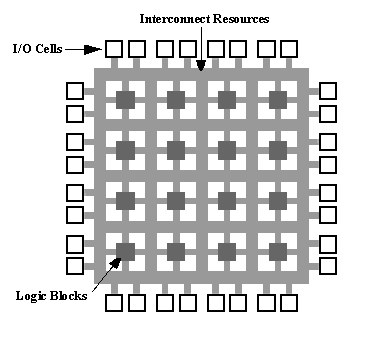
\includegraphics[width=0.5\textwidth,keepaspectratio=true]{./images/fpga1a.gif}
  \caption{Componentes de una FPGA}
  \label{fig:esquema}
 \end{center}
\end{figure}

		\subsubsection{\textcolor{orange}{Bloques Lógicos Configurables y Lookup Tables}}
Todas las \textit{FPGA} se basan en arrays de pequeños elementos de lógica digital. Los problemas de lógica digital se descomponen en circuitos lógicos que puedan ser mapeados a uno o más de estas “celdas lógicas” a través de un proceso llamado “technology mapping".

Cada bloque de logica configurable varia de acuerdo a su fabricante, en el caso de Xilinx tienen el nombre Logic cell (LC) contiene una 4 input LUT, un multiplexor y un registro. Se puede configurar la polaridad del clock, el clock enable y la señal de reset.


\begin{figure}[h!]
 \begin{center}
 %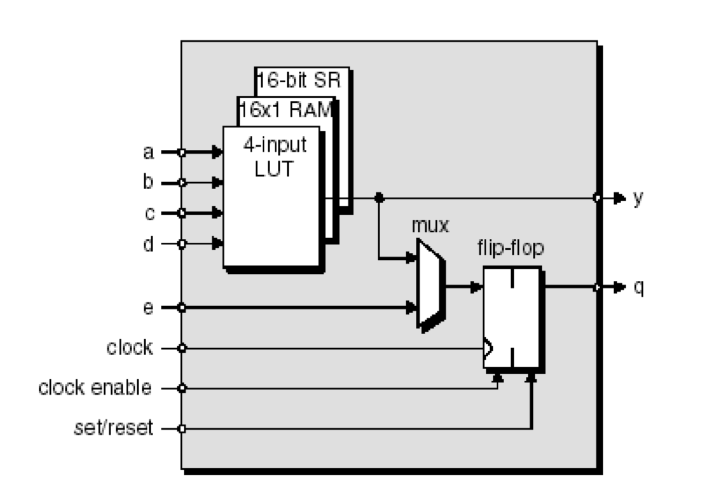
\includegraphics[width=0.5\textwidth,keepaspectratio=true]{./images/celda}
  \caption{Componentes de una FPGA}
  \label{fig:esquema}
 \end{center}
\end{figure}

También se encuentran las Lookup Tables, que son elementos lógicos que están compuestos de al menos un registro programable (flip\-flop) y alguna lógica de entrada, que usualmente está implementada como una lookup table de n entradas, donde n es 5 o menos. Estas LUTs son capaces de implementar cualquier función combinacional de sus entradas.

		\subsubsection{\textcolor{orange}{Bloques de Entrada y Salida de propósito general }}

Las FPGAs poseen pines TTL, CMOS, PCI, LVDS y muchos otros que les permiten hacer de interface y convertir muchas tecnologías diferentes. Las FPGAs tienen bloques de I/O dedicados para clocks y resets globales. También incluyen PLL y esquemas para el manejo de clocks permitiendo múltiples dominios del mismo.

Las FPGAs actuales tienen impedancias de I/O configurables,  permiten el uso de resistencias internas terminales cuyos valores pueden ser configurados por el usuario. 


		\subsubsection{\textcolor{orange}{Bloques de Memoria}}

Las FPGAs actuales incorporan memorias on-chip, tales como las SRAM. Estas memorias pueden ser accedidas en forma jerárquica, desde la memoria local de cada celda a la memoria global de los bloques compartidos de memoria. Si bien esto no hace a la esencia de la FPGA, todas hoy en día poseen estos bloques para dar solución al impacto que conlleva utilizar una memoria externa al chip, mayormente soluciona los problemas de latencia.

		\subsubsection{\textcolor{orange}{Multiplicadores}}
Algunas funciones como los multiplicadores son muy lentos si se implementan mediante la conexión de un gran numero de bloques lógicos. Por eso muchas FPGAs incorporan bloques multiplicadores hardware. Estos bloques se encuentran muy cerca de los bloques de RAM embebidos. 
\subsubsection{\textcolor{orange}{Manejadores de Clock Digitales}}
 Se llama clock tree porque la señal de clock principal es ramificada para que alcance a todos los flip-flops.Esta estructura es así para asegurarse que todos los flip flop estén lo mas cerca posible del clock y evitar el problema del skew.El clock tree es implementado usando canales separados de los de propósito general para interconectar los bloques.

		\subsection{\textcolor{orange}{Microprocesadores Soft-Core }}

El avance en la en la tecnología de fabricación de VLSI (Very Large Scale Integratio) a medida que se agregaron más y más transistores,y en consecuencia más y más funciones fueron integradas en un mismo chip, por lo tanto también las capacidades en FPGAs. Grandes diseños de sistemas digitales que fueron sólo para ser implementado como ASICs, luego tuvieron la opción de ser ejecutados en FPGA.

El microprocesador, ya sea como un componente discreto o  como parte de otra lógica en el mismo chip, es una candidato  para ser  implementado en FPGA. Esto introdujo un mayor potencial para la exploración del espacio de diseño haciendo que la logica de computo especifica sea implemetada junto con un microprocesador estándar %\cita{estiqueta20}
		
	\subsubsection{\textcolor{orange}{ IP-Core}}

El diseños de circuitos digitales se dividen normalmente en bloques funcionales, que se refiere como módulos, o \textit{cores}. Un \textit{core} estara formado por sub-bloques que ayudan a poner en práctica su funcionalidad. Los \textit{cores} pueden variar en tamaño hasta el tamaño total de un microprocesador. Un \textit{core} puede ocupar una FPGA entera al ser implementado, mientras que sólo se crea una instancia entre otros en una FPGA más grande o en un ASIC. Los \textit{núcleos} se describen generalmente utilizando un lenguaje de descripción de hardware (HDL) en un nivel de abstracción conocida como registro nivel de transferencia (RTL).

El proceso de tomar la descripción RTL de un diseño y convertirlo en un lista de primitivas o puertas lógicas y las conexiones entre ellos, dejando luego que la  implementación se realice en una tecnología de destino, se conoce como\textit{síntesis}. Analogamente a la compilación de software - que se tiene un programa en un lenguaje de alto nivel, como C, y  es convertido a codigo maquina. 

El resultado de la síntesis, conocida como una \textit{netlist}, está en un nivel de abstracción denominado nivel de la puerta.En pocas palabras, es esta lista de conexiones que se utiliza para su posterior procesamiento en una configuración para FPGA o en un diseño para ASIC.

Los cores pueden ser diseñados por una persona o entidad, los desarrolladores de \textit{cores} y licenciatarios varían en tamaño desde particulares a empresas de miles de millones de dólares. El producto, en este caso se conoce como un \textit{IP core  Intellectual Property Core} el diseño es la propiedad intelectual de los desarrolladores de terceros y la derecho a usarla recibe la licencia del cliente. La \textit{Intellectual Property IP} varia  de  acuerdo a las licencia.

			\paragraph{\textcolor{orange}{ Tipos de IP-Core}}
hard soft y intermedios
%El producto , en este caso se conoce como un núcleo IP (propiedad intelectual a menudocore) en el sentido de que el diseño es la propiedad intelectual de los desarrolladores de terceros y le da derecho a usarlo  recibe la licencia del cliente. Se utilizan los términos IP y el núcleo indistintamente y en combinación para significar la misma cosa .IP puede ser en una variedad de formas cuando licencia . Cuando está en la forma de sintetizable RTL entonces el IP se conoce como un núcleo blando . Si se trata de una forma menos abstraído forma , tal como un formato de un mensaje - diseño listo lista de conexiones o para la fabricación, que se conoce como IP núcleo duro .

\subsection{System on Chip}

La innovación continua en la tecnología de fabricación de semiconductores, ha visto al
disponible "real estate" en los chips de aumento en línea con la predicción de 1965 por Gordon E. Moore. La capacidad de los ingenieros de diseño digital para hacer uso de estos transistores adicionales no ha seguido el ritmo de este incremento en la capacidad de fabricación (21). El tiempo para las necesidades del mercado de estos diseños cadam vez más complejos ha permanecido estático, si no apretado.

Esto ha llevado a la aparición de la industria de núcleo IP compuesta de las empresas especializadas en el desarrollo y concesión de licencias IP a las personas la construcción de sistemas de FPGA o ASIC aplicación.

Esto permite a los equipos de diseño para montar un sistema formado por componentes básicos desarrollados por terceros para implementar el soporte para los protocolos de comunicación estándar, como Ethernet, IIC o SPI, mientras se concentra sus esfuerzos en el diseño de lo que es lo que hace que su diseño único o
particularmente valiosa


 intro,  deferencias entre micros soft y hard. fabricantes.ventajas de uno sobre el otro.
 Ejemplo:
En la industria existe un grupo ligeramente diferente de microprocesadores  Soft-Core , apuntando principalmente al hardware reconfigurable . Tres de los más grandes proveedores de FPGA , Xilinx , Altera y Lattice , ofrecen sus propios núcleos de microprocesadores RISC de 32 bits. Los dos mayores proveedores de dispositivos FPGA , Altera y Xilinx , proporcionan la Nios y Microblaze núcleos , respectivamente. Ellos se consideran hard-core en los que la fuente RTL no se encuentra  disponibles y sólo pueden ser implementadas en sus  Tecnologías FPGA .

Existe un grupo de cores opensource que no están limitados por la tecnología, y
son cores intrínsecamente soft . Los cores mas destacados en esta categoría son los  microprocesadores de 32 bits  SPARC LEON OpenRISC 1200 , y el núcleo LatticeMico32 de la empresa Lattice.

Para el desarrollo de una aplicación reconfigurable existe los micro cores de 32bist que ofrece los proveedores de las FPGA y los micro soft-core opensource disponibles de forma gratuita.

 Sin embargo , cuando se trata de ser capaz de desarrollar y vender un producto a base de estos núcleos , hay consideraciones adicionales sobre la concesión de licencias de los diseños. Estas cuestiones relacionadas con licencias voluntad se discutirá en una sección posterior.
%Las ventajas de un verdadero  sobre un soft-core y hard-core,%\ tienen que ver con la apertura del diseño, y la ausencia de restricciones sobre lo que se puede hacer con la obra. Con un diseño de la fuente verdaderamente abierta existe la opción de personalizar la descripción RTL para implementar la optimización o la funcionalidad deseada . Portabilidad y el producto se refiere al final de su vida también no surgir con la descripción RTL del diseño .


%%%%%%%%%%%%%%%%%%%%%%%%%%%%%%%%%%%%%%%%% CAPITULO 3 %%%%%%%%%%%%%%%%%%%%%%%%%%%%%%%%%

\section{\textcolor{orange}{Benchmark}}
Este capitulo lo puse para darle una intro a el estudio de los test que voy a poner en el estudio de los micor soft-core
	\subsection{\textcolor{orange}{Introducción}}
explico un poco para q los uso y en que se usan

En informática , un punto de referencia es el acto de ejecutar un programa de ordenador, un conjunto de programas , u otras operaciones , a fin de evaluar el rendimiento relativo de un objeto , normalmente mediante la ejecución de una serie de pruebas estándar y los ensayos en contra de ella . El término ' benchmark ' también se utiliza sobre todo para los fines de los propios programas de benchmarking elaboradamente diseñados.

Benchmarking se asocia generalmente con la evaluación de las características de rendimiento de hardware , por ejemplo , el rendimiento de punto flotante de funcionamiento de una CPU , pero hay circunstancias en que la técnica también es aplicable al software . Puntos de referencia de software están , por ejemplo, van en contra de los compiladores o sistemas de gestión de bases de datos .

	\subsection{\textcolor{orange}{CPU core benchmarking}}
 
A pesar de que no se corresponde con la forma en que utilizaría un procesador en una aplicación real , a veces es importante aislar el núcleo de la CPU de los otros elementos del procesador y centrarse en un elemento clave. Por ejemplo , es posible que desee tener la capacidad de hacer caso omiso de la memoria y los efectos de E / S y se centran principalmente en la operación de el pipeline. Este es el dominio de CoreMark . CoreMark es capaz de probar la estructura de pipeline básica de un procesador , así como la capacidad de prueba de lectura / escritura de operaciones básicas , operaciones de enteros y operaciones de control

	\subsection{\textcolor{orange}{CoreMark}}

CoreMark es un punto de referencia que tiene como objetivo medir el rendimiento de las unidades centrales de procesamiento ( CPU) utilizados en sistemas embebidos. Fue desarrollado en 2009 por Shay Gal -On en EEMBC y está destinado a convertirse en un estándar de la industria , en sustitución de la referencia Dhrystone anticuada . El código está escrito en código C y contiene las implementaciones de los algoritmos siguientes : procesamiento de lista ( encontrar y ordenar ) , Matrix (matemáticas) manipulación ( operaciones con matrices comunes ) , máquina de estados ( determinar si un flujo de entrada contiene números válidos ) y CRC

%%%%%%%%%%%%%%%%%%%%%%%%%%%%%%%%%%%%%%%CAPITULO 4%%%%%%%%%%%%%%%%%%%%%%%%%%%%%%%%%%%%

\section{\textcolor{orange}{Software OpenSource y Libre}}%julius
		\subsection{\textcolor{orange}{Deferencias}}%http://www.slideshare.net/wilberth1594/tesis-alex-8795926,julius
Una interpretación sencilla de lo que se entiende por el término \textit {open source} o \textit{código abierto}, cuando se utiliza en el contexto de la descripción de un programa de software o diseño de hardware , es que el codigo fuente  de alguna manera está disponibles a la vista. A pesar de que es un amplio y potencial término ambiguo, un común acuerdo sobre la definición está en un documento llamado  Open Source Definition (OSD), publicado por la Open Source Initiative (OSI).

 La definición no es una licencia de software libre en sí, si no algo que se utiliza para medir condiciones frente a la distribución, si se determina que cumplen con las condiciones, entonces se puede decir que es \textit{open source}. Lo que no es claro es lo que podría o debería ser hecho con una copia del código fuente.Cuando el software \textit{libre} o \textit{free} se utiliza para describir el software de código abierto, se refiere a los derechos y no al costo del usuario. La Fundación para el Software Libre (FSF) ofrece una definición para mostrar claramente qué se tiene que cumplir sobre el software para que pueda ser considerado libre (35). El termino Free Software Foundation (FOSS) es usado para referirse al software que se adhiere al OSD y FSF. El software \textit{libre} y de \textit{código abierto} es una sociedad inclusiva término que abarca tanto el software libre y software de código abierto que a pesar de describir modelos de desarrollo similares, tienen diferentes culturas y filosofías.

El software \textit{libre} se refiere a la libertad de los usuarios para ejecutar, copiar, distribuir, estudiar, cambiar y mejorar el software. El vocablo \textit{free} en ingles significa :gratis y/o libre. Por ello el término ha ocasionado confusiones dándose a entender, equivocadamente, que el software libre es gratuito o regalado. Pero no es una cuestión de presencia o ausencia de costo, puesto que el software libre no significa que no pueda ser comercial.

Stallman fundó la Free Software Foundation (FSF ) en 1985 para promover la libertad del usuario y para defender los derechos de todo el software libre( 28 ). La FSF patrocina el proyecto GNU. El software libre permite al usuario el ejercicio de cuatro libertades básicas:

\begin {itemize}
\item
 \textit{Libertad 0} Además el software \textit{libre} permite estudiar cómo funcionan y adaptarlo a las necesidades de quien lo use. Tener acceso a su código fuente posibilita, entre otras cosas, descubrir qué posibilidades tiene, etc. El adaptar el programa a las necesidades del usuario se puede suprimir partes que no le interesen, agregar otras partes que considere importantesm copiar una parte que realiza una tarea y/o adicinarla a otro programa, etc.

\item
\textit{Libertad 1} El software, sus copias y las modificaciones se pueden distribuir libremente, lo que significa poseer la libertad de redistribuir el programa, gratis o con algún costo, ya sea por mail, FTP, o en CD, redistibuyéndolo a una persona o a varias, a una persona que vive en otro país, etc.

\item 
\textit{Libertad 2} Es posible mejorarlo y hacer pública esas mejoras. La libretad de hacer un programa mejor, implica que se puede hacer menores los requerimientos de hardware para funcionar, que tenga mayores prestaciones, que sus requerimientos no sean tan altos, que tenga menos errores, etc. El poder liberar las mejoras al público quiere decir que si se realiza una mejora que permita un requerimiento menor de hardware, o que haga que ocupe menos espacio, se puede redistribuir ese programa mejorando o simplenete propoenr la mejora en lugar público (un foro de noticias, una lista de correo, un sitio web, un FTP, un canal de chat).

\item 
\textit{Libertad 3} El usuario al poseer el código fuente tiene poder de decisón, ya que podrá elegir quién puede modifica los programas que ha adquirido para mejorarlos (o bien mejorarlos el mismo). Es decir esto permite que no exista un monopolio, porque en el caso de que un software sea discontinuado el usuario podrá nuevamente (al poseer el código) elegir a un desarrollador para continuar utilizando el software que fue discontinuado. Además el usuario no estará completamente a merced de tener que renovar su hardware y software constantemente según ocurre a menudo con las políticas de las empresas que producen software privativo y también será libre de vender o redistribuir software libre.
 
 \end {itemize}
 
Mediante la licencias un autor permite el uso de su creación a otras personas, de la manera que el cree aceptable. En ese sentido la licencia es el intrumento que regula las maneras en que el usuario puede utilizar el software.

También una licencia de software es un contrato que determina en qué condiciones el usuario puede utilizar el programa informático y qué obligaciones asquiere para su uso. Cuando se instala un programa informático, o a veces, incluso, por el simple hecho de abrir el sobre que lo contiene, se esta aceptando las condiciones de su licencia de software.

Cuando IBM comenzó la venta de computadoras a gran escala en la década de 1960, el software venia incluido como código fuente. Una década más tarde, sin embargo, comenzaron a "desagregar"  el software, y se convirtió en habitual para los fabricantes de computadoras, no solo limito  el uso del mismo código fuente a los competidores, sino que también elimino la capacidad de modificar el código libremente y compartirlo%\cita{}(26).  

La licencia División de Software de Berkeley (BSD) y la Pública General del proyecto GNU (GNU GPL) son dos de las primeras licencias de código abierto. Ambos proporcionan la libertad de usar software de código fuente abierto para cualquier propósito y permitir la modificación y la distribución de su código fuente sin tener que pagar regalías. Las diferencias entre los dos pone de relieve una diferencia ideológica entre los defensores del código abierto .

Un punto significativo de diferencia entre las licencias BSD y GPL es que este último le permite
\textit{modificar su copia o copias del Programa o cualquier parte de el, y copie
y distribuir tales modificaciones ... supuesto que además ... hace que la
totalidad de cualquier trabajo que distribuya o publique y que en todo o en
parte contenga el Programa o cualquier parte del mismo, ya sea con o sin
modificaciones, para ser autorizadas sin cargo alguno para terceras partes bajo el
términos de esta Licencia Pública General.(GPLv1) ( 29 ). } %\cita{}

La GNU GPL se conoce como una licencia \textit{viral}, en que cualquier diseño haciendo uso de código ya licenciado bajo la GNU GPL debe ser entonces licenciado bajo la
GNU GPL o cualquier licencia juzgados como igualmente sin restricciones por la FSF. En pocas palabras, una condición de uso del código licenciado bajo GPL es que su diseño se debe tener licencia bajo la GPL o una licencia compatible. Las licencias que se consideran compatibles con la GPL por la FSF son generalmente similares en las libertades que garantiza el software libres. La licencia se transmite al código que hacen uso de ella. El GNU GPLv3 exige que cuando un proyecto adopta esta licencia el código fuente debe estar disponible y que las patentes o derechos digitales (DRM) no inhiben a otros del uso del diseño. 

La licencia BSD modificada es básicamente la misma que la original sin la clausula de publicidad. De acuerdo con dicha cláusula, todo el material de publicidad en el cual se menciona características o la utilización de este software tenia que mostrar el siguiente asentimiento:"este producto incluye software desarrollado por la Universidad de California, Berkeley y sus contribuyentes ".

Esta cláusula de publicidad no permitía que fuera compatible con la lincencia GPL pero a partir de su versión 2.0 fue eliminada y la licencia pasó a ser compatible con la GPL.

La GNU GPL es en cierto modo, más restrictiva que la licencia BSD sobre las libertad de hacer lo que uno quiere con el código fuente. En la GNU se estipula que el código modificado debe estar disponible, y cualquier diseño utilizado con código GPL tiene también que venir bajo la GNU GPL. Sin embargo, esto no es diferente a cualquier licencia comercial, donde el código fuente escrito por un empleado de una empresa,o todo el código que se modifican o crean esta bajo la licencia exclusiva de la empresa. En el caso de la licencia de GNU, sin embargo, los usuarios están obligados a mantener su diseño abierto y libre como la GPL de GNU hace, de la misma manera el empleado de la empresa está obligado a mantener su código propietario en secreto para cualquiera que no sea de la  empresa.

Otro punto de controversia es el uso combinado de los diseños en los que cada uno es bajo
una licencia diferente , y ha dado lugar al concepto de compatibilidad de la licencia . El significado
de uso aquí es ambiguo y depende del contexto , sin embargo, en este ejemplo, será
implicar el uso de un formato de la versión binaria precompilada de un diseño. En el caso de que uno
diseño utiliza una biblioteca binaria GPL , aunque no de origen se ve o se modifica
el usuario del diseño GPL , la GNU GPL especifica que no se puede utilizar a menos
el otro diseño está también bajo la GPL. El uso de las bibliotecas precompilados , compuesto
de funciones comunes , en los programas informáticos es muy común y es equivalente a la
ejemplo dado aquí . En el caso de que una biblioteca es bajo la GPL , cualquier cosa que utiliza
él ( también conocida como la creación de un vínculo a la biblioteca, o la vinculación con la biblioteca ) debe
también vienen bajo la GPL.
Sin embargo , la cuestión de la inclusión real en una aplicación compilada
Binario GPL (conocido como la vinculación estática ) no es tan contencioso - esto se considera
para ser el equivalente de la inclusión y la compilación de la fuente original - el debate
es sobre la vinculación dinámica. Esto implica el uso de una biblioteca de software precompilado que residen
en otro lugar ( no dentro de una aplicación compilada ) cuando se ejecuta una aplicación .
Si un programa que vincule dinámicamente a una biblioteca se considera un derivado
el trabajo es un tema debatido. El Proyecto GNU considera estas aplicaciones como derivado
obras y requiere que se adhieran a los requisitos de la licencia GPL de GNU .
Una visión alternativa es que estos programas utilizan la vinculación dinámica no son derivados
obras ( 30 ) ( 31 ) . Una solución para aquellos que deseen escribir bibliotecas , y no tienen la
interpretación más estricta de la obra derivada se les aplica , a propuesta de la GNU
Proyecto en su poca licencia de uso general ( LGPL ) . Se trata de un trade-off , lo que permite
para demostrar que la tecnología licenciada Proyecto GNU es de alta calidad y
fomentando así la participación de las personas en el proyecto, al tiempo que conserva algo de
sus requisitos de libertad . El Proyecto GNU , sin embargo , prefiere a los desarrolladores liberan
bibliotecas bajo la GPL , lo que obliga a quienes lo utilizan para su trabajo contribuyen a
el cuerpo de la GNU GPL licencia de software.


El objetivo del Proyecto GNU de implementar un operativo completamente libre y gratuito
sistema , se avanza a buen ritmo en la década de 1990 , pero le faltaba el nivel más bajo llave
componentes . En ese momento un estudiante universitario finlandés, Linus Torvalds, había escrito
un núcleo de reemplazo ( componente de interfaz de hardware central de un sistema operativo )
para Minix , un sistema operativo de tipo Unix bajo costo mínimo restringido a
uso educativo solamente. Una vez kernel Torvalds había llegado a un estado relativamente estable el
aplicaciones del sistema operativo de MINIX fueron reemplazados por los disponibles
por el Proyecto GNU. Torvalds vuelva a autorizar el núcleo ( como el propietario del copyright
esto era admisible ) a la GNU GPL y el primer funcionamiento y totalmente GNU
Sistema operativo GPL vino a la existencia ( 32 ) .

La combinación del núcleo de Torvald , conocido como el kernel Linux y el GNU
Aplicaciones y bibliotecas de software del proyecto se ha convertido en el servidor más utilizado
sistema operativo en el mundo.

Su adopción entre escritorio , estación de trabajo y plataformas móviles no es tan alto , pero son
aumentando rápidamente a medida que los paquetes del sistema operativo , conocido como distribuciones o simplemente
distribuciones , cada vez más ampliamente disponibles y proporcionar equivalentes , si no mejor , el usuario
experiencias que los sistemas operativos propietarios 

 Ejemplos de otros exitosos y ampliamente adoptado proyectos de código abierto son el servidor web Apache , la oficina de los servicios públicos paquete OpenOffice.org y el proyecto Mozilla, que crea software de correo electrónico y navegador web. A pesar de que esta última pareja no eran originalmente de código abierto, el lanzamiento de su código fuente bajo licencias de código abierto fue significativa, y continúan los proyectos populares de la actualidad 

A medida que la popularidad y la utilidad de Internet ha crecido , también lo han hecho en línea
comunidades por diversas causas 
La captación de Internet y la comunicación en línea proporcionan la chispa para la gran fuente abierto
comunidades. En cualquier caso, lo que ha dado como resultado es un sinnúmero de comunidades y sueltos tejer
grupos que contribuye a abrir el desarrollo fuente de casi cualquier cosa.

Sitios web de gran tamaño para que las comunidades se centraron en el desarrollo de software de aplicaciones informáticas ,
como SourceForce , freshmeat , Ohloh y hacia arriba de acogida CPAN de decenas de
miles de proyectos . Un grupo llamado Freenode proporciona Internet Relay Chat ( IRC )
servidores donde decenas de miles de desarrolladores de código abierto se reúnen para interactuar .

Hay una serie de pequeños servicios de alojamiento de proyectos libres dirigidos a grupos
desarrollo de software como Google Code , Launchpad , GitHub , GNU Savannah,
así como los sitios de la comunidad antes mencionados .

Un sitio, comenzando justo después de que el año 2000 , llamado OpenCores centra en proporcionar
un sitio para la comunidad de hardware de código abierto. Fue de los primeros en
proporcionar a la comunidad de desarrollo de hardware y es actualmente el más grande , con
más de cien mil usuarios y cerca de mil proyectos

Software como software multimedia avanzada, de productividad de oficina , gráficos herramientas , sistemas operativos y software de comunicaciones tienen alternativas de código abierto , desarrollado en el abierto, y por lo general libre para descargar y utilizar. Los gobiernos y las grandes empresas están aprovechando cada vez más software de código abierto existente y se están convirtiendo en importantes contribuyentes a los proyectos del software que adoptan. Las tendencias recientes han hecho mucho para disipar la imagen de la legión de solitarios desarrolladores de código abierto que son los únicos contribuyentes de trabajo. Como las grandes entidades comerciales aumentan su adopción y utilización de los proyectos de software libre, que se están convirtiendo , por el momento, los contribuyentes más frecuentes. El kernel de Linux tiene ahora la mayor proporción de sus contribuciones de código vienen no de los aficionados o entusiastas individuales, sino en lugar de las entidades comerciales ya sea trabajando con el núcleo Linux en sus productos, tales como Red Hat, o que deseen asegurar el apoyo a su hardware en el kernel, tales como Intel , AMD e IBM. Lo mismo es cierto para proyectos como Apache y MySQL.

La gran cantidad de software de código abierto disponible ofrece la elección entre
la adopción de software libre , pero con el lanzamiento de su obra derivada, y el desarrollo de una solución interna o la compra de una solución propietaria y revelando el trabajo no uno . El proyecto GNU GCC y binutils , el desarrollo del AM y el mantenimiento está siendo realizado en gran parte por los empleados por las empresas que tienen interés en mantener el apoyo o las plataformas en las mejores condiciones . La salud del proyecto y, a continuación , obviamente,
es impulsado por el uso generalizado de las herramientas del CCG , que es debido a la fuerte inicial aplicación . El aumento del potencial comercial del software de código abierto tiene resultado en empresas aportando recursos a estos proyectos en lugar de , el desarrollo de y el mantenimiento de su propia suite compilador de propiedad en el caso de GCC , por ejemplo . Este es uno de los objetivos de los creadores de código abierto - para proporcionar una base del software de código abierto tan rico que los desarrolladores están en mejor situación y la adopción de software libre liberación de su obra derivada y por lo tanto el aumento de la masa existente de software en lugar de desarrollar desde cero o comprar una solución propietaria.
Aunque sólo se ha descrito aquí , las motivaciones para la adopción y contribuir a código abierto podrían ser muchas y variado y dependerá en gran medida de la funcionalidad real de la fuente abierta 

No hay duda de algún tipo de software de gran utilidad se ha escrito y contribuido
para abrir proyectos de software , sin embargo fuente abierta no debe ser visto como un innovador
fuerza , en lugar de un paso en el camino hacia una mayor mercantilización de la tecnología.
El espíritu empresarial y el afán de lucro por lo general conducen al alto riesgo y alta innovación
las empresas que participan en la implementación de la tecnología de corte del borde 

Una de las motivaciones para el desarrollo de código abierto desde el punto de vista comercial,
como ya se ha eludido a , proviene de la capacidad de proporcionar y cobrar por servicios
en relación con el proyecto de código abierto. A pesar del hecho de que el IP está disponible públicamente ,
implementar o personalizar el proyecto normalmente requiere experiencia en el correspondiente
disciplina y con el proyecto en particular. Las empresas adoptar y mantener un
solución de código abierto por lo general tienen sólo el costo de los conocimientos necesarios para hacerlo, con
sin regalías o licencias adicionales tasas que se pagan

en la actualidad hay alternativas de código abierto para los sistemas de software de TI de propiedad de hace cinco o diez años , lo que resulta en el costo de la misma funcionalidad ahora es sólo el personal de apoyo especializado necesario.
Esta necesidad de conocimientos potencialmente podría ser compartida entre el personal y el apoyo de la casa
los trabajadores contratados a consultores especializados, o incluso desarrolladores del proyecto
a sí mismos . En resumen, los desarrolladores de código abierto renunciar a ciertas reclamaciones sobre
la IP , lo que potencialmente gran parte no era su propia idea o considera especialmente
innovadora , para empezar, la recompensa en forma de empleo continuado realizando
servicios relacionados con el proyecto.

A pesar de fuente abierta no es un controlador tradicional a la innovación no se opone a
que de ser la estrategia de desarrollo elegida para una tecnología innovadora .
Cualquier diseño bastante innovador suele verá retornos valiosos para la inversión necesaria para llevarla a cabo . Sin embargo, con alternativas de código abierto que brotan de forma relativamente rápida , su ventaja no puede durar por mucho tiempo ya que otros toman nota de lo que han hecho desarrollos innovadores y si , hay que vale la pena en forma de soluciones de código abierto. Puede llegar a ser una opción para el desarrollador si persiguen el desarrollo de código abierto , para empezar , en base a la duración de una ventaja competitiva se puede mantener con una implementación propietaria frente a la capacidad de proporcionar apoyo a largo plazo para una aplicación que potencialmente ver más utilizar ( la versión de código abierto. ) lo mejor de ambos mundos puede ser un buen método , donde inicialmente el producto está autorizado por una cuota, antes de liberar el código fuente que permite a otros a desarrollar y espero mejorar el proyecto. Como producto es el ciclo de la vida llega a su fin , puede ser ventajoso para liberar la fuente
para permitir que cualquier usuario ampliados para solucionar los problemas derivados de la plataforma inevitable
cambios que se producen . Todavía hay un problema aquí, sin embargo , como la implementación propietaria mantiene su dominio , mientras que no hay , una fuente equivalente abierto ,
el diseñador nunca puede elegir para liberar la fuente , pero entonces se corre el riesgo de un diferente
aplicación con funciones equivalentes ganando más popularidad , y por lo tanto
el diseñador original es vida , pero no idea sobre su capacidad para proporcionar apoyo a la misma .


Esta breve mirada a la situación actual de código abierto ha indicado que el código abierto
se ha convertido en una fuerza a tener en cuenta en el mundo del software , pero este es sin duda
no es el caso en la actualidad para el desarrollo de hardware de código abierto. Las razones de esto se
ser explorado en los tramos finales . Sin embargo , el enfoque moderno de código abierto
el desarrollo y los beneficios y las motivaciones de la misma se presentaron e indican
sin duda hay un caso para la adopción del enfoque de desarrollo de código abierto. allí
hay duda de que habrá seguir aumentando la adopción del código abierto
desarrollo y modelo de licencia en el futuro. A medida que la cantidad de abierto disponible
aumenta diseños de origen , y la comprensión de los márgenes de aproximación , lo hará
seguramente continuará para demostrar que es un enfoque valioso para el desarrollo de
tecnología
%Conclusión!!Trabajar con un sistema final bajo licencias de hardware siguiendo el modelo de la Licencia LGPL para el software. Estamos comprometidos con el ideal de libre disposición, de libre uso y hardware de código abierto reutilizable.

Una interpretación sencilla de lo que se entiende por el término \textit{open source}, cuando se utiliza en la contexto de la descripción de un programa de software o diseño de hardware, es que el diseño Fuentes de alguna manera están disponibles a la vista. A pesar de que es una amplia y potencialmente término ambiguo , un común acuerdo sobre la definición está en un documento llamado la Open Source Definition (OSD ), publicado por la Open Source Initiative (OSI ) 

La definición no es una licencia de software libre en sí , más bien algo para medir condiciones de distribución frente para determinar si cumplen y , si lo hacen, entonces se puede decir a ser de código abierto ( 36 ) . Lo que no es inmediatamente claro es lo que podría o debería ser hecho con una copia de la fuente de diseño , práctica y legalmente. Cuando el software libre se utiliza para describir el software de código abierto , se refiere no al costo para el usuario, pero los derechos del usuario. La Fundación para el Software Libre (FSF ) ofrece una definición para mostrar claramente qué debe cumplir sobre una pieza de software para que pueda ser considerado libre ( 35 ) .

El software libre de código abierto plazo ( FOSS) se usa para referirse al software adherirse tanto al OSD y FSD . El software libre y de código abierto es una sociedad inclusiva término que abarca tanto el software libre y software de código abierto que , a pesar de describir los modelos de desarrollo similares , tienen diferentes culturas y filosofías.
El software libre se enfoca en las libertades filosóficas que da a los usuarios, mientras que abierto origen se centra en las fortalezas percibidas de su modelo de desarrollo peer-to -peer ( 37 ) ( 38 ) .



la intro al tema contando un poco  las comunidades de codigo abierto y por ulitmo de OpenCore

Ejemplo: 
A medida que la popularidad y la utilidad de Internet ha crecido , también lo han hecho las comunidades de opensource.
La comunicación fue el inicio para las grandes comunidades de opensource. Lo que  dio como resultado un sinnúmero de comunidades y grupos que contribuye a abrir el desarrollo fuente de casi cualquier cosa.

Sitios web de gran tamaño para que las comunidades se centraron en el desarrollo de software de aplicaciones informáticas , como SourceForce , freshmeat , Ohloh y hacia arriba de acogida CPAN de decenas de miles de proyectos . Un grupo llamado Freenode proporciona Internet Relay Chat ( IRC ) servidores donde decenas de miles de desarrolladores de código abierto se reúnen para interactuar .

Hay una serie de pequeños servicios de alojamiento de proyectos libres dirigidos a grupos desarrollo de software como Google Code, Launchpad, GitHub, GNU Savannah,
así como los sitios de la comunidad antes mencionados.

OpenCores es  sitio/ comunidad más grande para el desarrollo de los  IP core de hardware como de código abierto del mundo.
OpenCores.org proporciona el código fuente de los diferentes proyectos HW digitales (IP-cores, SoC, boards, etc) y apoyar a los usuarios con diferentes herramientas, plataformas, foros y otras informaciones útiles. 

	%	\subsection{\textcolor{orange}{Deferencias}}%http://www.slideshare.net/wilberth1594/tesis-alex-8795926,julius
Aca vamos a poner las libertades que permiten uno y otro
		\subsection{\textcolor{orange}{GPL}}

GPL es que el
este último le permite modificar su copia o copias del Programa o de cualquier porción de él , y copiar y distribuir esa modificación ... supuesto que además ... hacer que el
totalidad de cualquier trabajo que distribuya o publique y que en todo o en
parte contiene el Programa o cualquier parte del mismo , ya sea con o sin
modificaciones, para ser autorizadas sin cargo alguno para terceras partes bajo el
términos de esta Licencia Pública General. ( GPL v1 ) ( 29 )

La GNU GPL se conoce como una licencia viral , en que cualquier diseño haciendo uso de código ya licenciado bajo la GNU GPL debe entonces , sí , ser licenciado bajo la GNU GPL o cualquier licencia juzgados como igualmente sin restricciones por la FSF. En pocas palabras, una condición de uso del código licenciado bajo GPL es que su diseño se debe tener licencia bajo la GPL o una licencia compatible. Licencias considerarse compatibles con la GPL por la FSF son generalmente similares en las libertades que garantiza el software. En otra.
Es decir, que se ven obligados a compartir, si piensas que no, y ser objeto de la licencia de GNU, o un equivalente aprobado . La licencia , en efecto, infecta elcódigo que hacen uso de ella. El GNU GPLv3 exige que cuando un proyecto adopta esta la licencia del código fuente debe estar disponible y que las patentes o derechos digitales (DRM ) no inhiben a otros del uso del diseño

La GNU GPL está en cierto modo, irónicamente, más restrictiva que la licencia BSD
sobre las libertad de hacer lo que uno va con el código fuente . En él se estipula la
código modificado debe estar disponible , y cualquier diseño utilizado con código GPL debe
también vienen bajo la GNU GPL.

Sin embargo, esto no es diferente a cualquier licencia propietaria , escrito por un empleado de una empresa, todo el código que modifican o crean viene en la empresa , licencia propietaria marca. En la licencia GNU, caso del AM , sin embargo , los usuarios se ven obligados a mantener su diseño abierto y libre como la GPL de GNU hace que , de la misma manera que el empleado está obligado a mantener su código propietario y secreto para nadie que no sea de la compañía .
		\subsection{\textcolor{orange}{LGPL}}
%Revisemos este título -- PABLO JULIUS :P
		\subsection{\textcolor{orange}{OpenSource}}
intro a opensource

EJ
La apertura del código de la propiedad intelectual desarrollada para el proyecto OpenRISC, y otros en OpenCores, ha sido a la vez un obstáculo y una ayuda, pone a la vista el estado de el desarrollo, pero es útil, ya que permite que cualquiera pueda participar en el continuo desarrollo de cores. %\Esta sección discutirá los pros y los contras del opensource
		

		\subsection{\textcolor{orange}{¿Quien tiene el Hardware?}} 

la idea es poner pro y contra de trabajar con open source
EJ
El uno de los problemas que enfrentan los desarroladores del opensource que no lo tiene lo desarrolladores  de software es la necesidad de usar plataformas privativas para implementar el diseño.Estas plataformas que como elemento base una FPGA, contienen múltiples periféricos ICs , que tienen que ser comprados , así como la depuración y la programación de hardware.
Se suma a esto que generalmente las complicadas herramientas de programación de los proveedores, 
%así como el desarrollo de hardware curva de aprendizaje relativamente empinada impone a los principiantes , y no es demasiado sorprendente que técnicamente bien las personas que deseen participar en un proyecto de código abierto podrían elegir un software proyectar sobre un proyecto de hardware casi siempre.
 %También es cierto que la utilidad de cualquier diseño de hardware que se podría implementar en FPGA está limitado por el hecho de que se que se hace a un muy bajo nivel de abstracción, y para lograr cualquier resultado " útil" para un experimentador o aficionado, que por lo general requiere una gran cantidad de trabajo a lo largo de muchos niveles de abstracción para lograr algo que es fácilmente utilizable a partir de una interfaz en un modernoPC . Un ejemplo podría ser el desarrollo de un núcleo para llevar a cabo no estándar 
%\I / O con las transacciones de un sensor u otro boutique de IC, para proporcionar información a un programa de asistencia en la automatización del hogar , o el control de un modelo a escala y la similares. Esto requeriría el desarrollo y prueba del modelo de hardware y implementación en FPGA . Suponiendo que no era un microprocesador está ejecutando en ese FPGA proporcionar servicios de red a través de un RTOS , este nuevo módulo personalizado haría luego exigir su capa de software desarrollado , lo que significa que un conductor, y la satisfacción de diversas Ganchos de nivel operativo en la aplicación que se ejecuta en la FPGA , el AM microprocesador, a proporcionar los datos a través del enlace de red . Sólo entonces sería este sensor , los datos del AM y luego estará disponible para la aplicación de nivel superior. Este es sólo un ejemplo en el que , muy probablemente el diseñador podría haber elegido una solución que utiliza un bus estándar, sin embargo no , el AM con frecuencia casos de control personalizado o núcleos de interfaz en FPGAs para proporcionar el acceso a la herencia , o las normas de muy nuevas o esotérica de autobús, y pone de relieve el extra trabajo que se requiere más allá de la escritura RTL para proporcionar la interfaz física. en vista de la cantidad de desarrollo y pruebas requeridas para poner en práctica estas soluciones típicamente , sería fácil sentirse abrumado por la cantidad de trabajo necesario para completar una tarea tan aparentemente trivial.

%Compare esto con el trabajo que participan en empezar a trabajar en una fuente abierta proyecto de software , que normalmente consisten en la descarga de una fuente de desarrollo árbol y el edificio ( en minutos ) que el proyecto con herramientas de desarrollo ya incluidos , o fácilmente obtenido , en el sistema operativo . La aplicación puede entonces ser
%ejecutar en el sistema host para comprobar la funcionalidad y el ciclo de desarrollo en gran medida termina allí. Las diferencias son el acceso inherentes a la plataforma de desarrollo ( el máquina host) , las herramientas de desarrollo más simples ( gcc, make en el sistema host ) y el ciclo de desarrollo y pruebas más corto y más fácil (que se ejecuta en el equipo host a través de un shell. ) 
%A medida que se desarrollan los proyectos de hardware de código abierto más y más ágil sistemas de desarrollo se ponen en su lugar , se puede esperar que estas barreras a entrada se convertirá disminuido . Los primeros días de desarrollo de software de código abierto habría parecido igual de difícil y laborioso . Con el tiempo , sin embargo , mejoras en los proyectos de forma en que se organizan y las herramientas utilizadas para su desarrollo , se han producido. La cantidad de software de código abierto disponible ha crecido y sigue hacerlo a un ritmo creciente . Se puede esperar que con el tiempo y el aumento participación , hardware de código abierto permitirá alcanzar un éxito similar .
		

		\subsection{\textcolor{orange}{OpenRISC}}

aca vamos a poner el objetivo del proyecto openRisc 

EJ:
 La mayoría de los proyectos de software libre tienen por objeto poner en práctica soluciones relativamente bien conocidas de una manera que permite la apertura y elimine las restricciones que se encuentran en otra implementaciones propietarias . 

El objetivo del proyecto OpenRisc de codigo abierto es proporcionar algo útil , productivo y abierto.
Los objetivos de estos proyectos de código abierto por lo general están alineados. 
Por ejemplo , considere el éxito obtenido por el proyecto del kernel de Linux, con miles de colaboradores y decenas de empresas que participan regularmente
en el desarrollo . El kernel Linux compite claramente con el propietario variantes de UNIX y de los productos de Microsoft y Apple  en todos los casos está experimentando un enorme éxito.
%\Para un proyecto como OpenRISC , un objetivo puede ser el uso generalizado entre los vendedores que  Actualmente utilizar procesadores por el líder de la industria , ARM , por su microprocesador sistemas basados ​​en . Por las razones que ya se ha esbozado sobre la verificación de abierto IP de origen y de los riesgos que implica , este tipo de absorción es poco probable que suceda en su actual estado, sin embargo eso no quiere decir que nunca pudo. En el momento de la OpenRISC de creación, los observadores indicaron que la IP de origen abierto podría convertirse en un jugador importante en la industria, si se hace bien ( 43 ) . Podría ser el caso que para los diseños que son en gran medida re- implementaciones de la tecnología conocida , los fundamentos de lo que son 25 - años de edad, de desarrollo de código abierto es un enfoque realista . Esto podría potencialmente conducir a menores costos ASICs , y por lo tanto la electrónica de consumo de bajo costo , como las regalías se eliminan , y los equipos de ingenieros la tarea de implementar en la casa controladores o microprocesadores, en lugar de trabajar para implementar y apoyar un un diseño de gran parte superflua , o bien podría ser la tarea de perfeccionar las partes específicas del el procesador de código abierto para lograr una mayor eficiencia en su aplicación, o sea reprogramado por completo el diseño más innovador IP .
%Es muy probablemente el caso , sin embargo, que se trata de un escenario de " crear y ellos vendrá " . Es poco probable que un esfuerzo concertado entre los desarrolladores de propiedad intelectual sería ocurrir espontáneamente . Incluso si fuera a aparecer de la talla de las universidades y casas de investigación financiados por el gobierno , la probabilidad del capó de desarrollar microprocesador diseños de atraer la atención de las casas de ASIC , a continuación, estimulando el desarrollo colaborativo , es baja. Los factores ya discutidos , como la dificultad de garantizar su diseños y altas barreras de entrada debido al costo y la experiencia están ahí, pero también restricciones sobre el tipo de información necesaria para perfeccionar implementaciones ASIC - biblioteca de tecnología específicos de las propias plantas de fabricación , que están estrechamente secretos guardados y con pocas probabilidades de ser liberados para los proyectos de código abierto para preparar los diseños para . Es probable que haya una distinción para dibujar aquí, también, entre los ASICs derivados su ventaja competitiva de su microprocesador o de otra medida IP . Potencialmente, las que se basan en un procesador del borde inferior de corte podría ser feliz de ayudar a contribuir a un proyecto de desarrollo de código abierto para un microprocesador, ayuda aportando horas de ingeniería para la verificación y tal vez incluso la adición de características , con el fin de evitar el pago de regalías que podría reducir su coste por unidad .



%%%%%%%%%%%%%%%%%%%%%%%%%%%%%%%%%%%%%%%%%%%%%%%CAPITULO 5%%%%%%%%%%%%%%%%%%%%%%%%%%%%%%%%%%%%%%%%%%%


	\section{\textcolor{orange}{Microprocesadores Soft-Core}}
	\subsection{\textcolor{orange}{LEON3}}
		\subsubsection{\textcolor{orange}{Características}}
		\subsubsection{\textcolor{orange}{Benchmarking}}
	\subsection{\textcolor{orange}{OpenRISC}}
		\subsubsection{\textcolor{orange}{Características}}
		\subsubsection{\textcolor{orange}{Benchmarking}}
	\subsection{\textcolor{orange}{Nios II}}
		\subsubsection{\textcolor{orange}{Características}}
		\subsubsection{\textcolor{orange}{Benchmarking}}
	\subsection{\textcolor{orange}{MicroBlaze}}
		\subsubsection{\textcolor{orange}{Características}}
		\subsubsection{\textcolor{orange}{Benchmarking}}

\section{\textcolor{orange}{Análisis de el OpenRISC }}
		\subsection{\textcolor{orange}{Arquitectura}}
		\subsection{\textcolor{orange}{Implementación}}
			\subsubsection{\textcolor{orange}{ORPSoC}}
			\subsubsection{\textcolor{orange}{MinSoc}}
		\subsection{\textcolor{orange}{Toolchain}}
		\subsection{\textcolor{orange}{Software}}
			\subsubsection{\textcolor{orange}{Librerías}}
			\subsubsection{\textcolor{orange}{Sistema Operativo}}
			
%%%%%%%%%%%ESTUDIO DEL PROBLEMA%%%%%%%%%%%%%%%%
	
\section{\textcolor{orange}{Estudio del Problema}}
	\subsection{\textcolor{orange}{Introducción}}
	\subsection{\textcolor{orange}{Requerimientos del Usuario}}
			\subsubsection{\textcolor{orange}{En cuanto al Hardware}}
			\subsubsection{\textcolor{orange}{En cuanto al las licencias}} 
			\subsubsection{\textcolor{orange}{En cuanto Sistema Operativo}} 	 
				 		\subsection{\textcolor{orange}{Estudio de componentes y de la viabilidad para el proyecto}}	
		\subsubsection{\textcolor{orange}{Objetivo}} 	 
		\subsubsection{\textcolor{orange}{Comparación de los Soft-Core}} 
	 	\subsection{\textcolor{orange}{Conclusiones de la elección del micro Soft-Core}}
 		\subsubsection{\textcolor{orange}{Placas de Desarrollo}}
			\paragraph{\textcolor{orange}{Xilinx}}
			\paragraph{\textcolor{orange}{Digilent}} 	 
			\paragraph{\textcolor{orange}{Altera}}
 		\subsubsection{\textcolor{orange}{CONCLUSIONES DE LA ELECCIÓN DE LA PLACA DE DESARROLLO}}
 		\subsubsection{\textcolor{orange}{SELECCIÓN DE LAS HERRAMIENTAS DE DESARROLLO}} 	 
 		\subsubsection{\textcolor{orange}{Elección de Sistema Operativo}}
%\paragraph{\textcolor{orange}{}}
			
\section{\textcolor{orange}{Requerimientos y Riesgos Del Sistema}}

\section{\textcolor{orange}{Implementación}}
	\subsection{\textcolor{orange}{Introducción}}
	\subsection{\textcolor{orange}{Arquitectura}}
%Criterios para la realización de testing  (o algo asi) -- PABLO JULIUS :P
	\subsection{\textcolor{orange}{Criterio para la realización de testing}}
	\subsection{\textcolor{orange}{Entorno de ejecución}}
		\subsubsection{\textcolor{orange}{Entorno de ejecución Standalone}}
		\subsubsection{\textcolor{orange}{Entorno de ejecución linux}}
	\subsection{\textcolor{orange}{PROTOTIPO UNO: Implementación del SoC MinSoc en FPGA}}
		\subsubsection{\textcolor{orange}{Introducción}}
		\subsubsection{\textcolor{orange}{Requerimientos del prototipo}}
		\subsubsection{\textcolor{orange}{Implementación}}
			\subsubsection{\textcolor{orange}{Diagrama de Secuencia}}
			\subsubsection{\textcolor{orange}{Testing}}
		\subsection{\textcolor{orange}{Conclusión}}
	\subsection{\textcolor{orange}{PROTOTIPO DOS: Implementación del SoC OrpSoc en FPGA}}
		\subsubsection{\textcolor{orange}{Introducción}}
		\subsubsection{\textcolor{orange}{Requerimientos del prototipo}}
		\subsubsection{\textcolor{orange}{Implementación}}
			\subsubsection{\textcolor{orange}{Diagrama de Secuencia}}
			\subsubsection{\textcolor{orange}{Testing}}
		\subsection{\textcolor{orange}{Conclusión}}
	\subsection{\textcolor{orange}{PROTOTIPO TRES: Implementación del SoC OrpSoc en FPGA con Sistema Operativo eCos}}
		\subsubsection{\textcolor{orange}{Introducción}}
		\subsubsection{\textcolor{orange}{Requerimientos del prototipo}}
		\subsubsection{\textcolor{orange}{Implementación}}
			\subsubsection{\textcolor{orange}{Diagrama de Secuencia}}
			\subsubsection{\textcolor{orange}{Testing}}
		\subsection{\textcolor{orange}{Conclusión}}
	\subsection{\textcolor{orange}{PROTOTIPO tres: Implementación OrpSoc en FPGA con Linux}}
		\subsubsection{\textcolor{orange}{Introducción}}
		\subsubsection{\textcolor{orange}{Requerimientos del prototipo}}
		\subsubsection{\textcolor{orange}{Implementación}}
			\subsubsection{\textcolor{orange}{Diagrama de Secuencia}}
			\subsubsection{\textcolor{orange}{Testing}}
		\subsection{\textcolor{orange}{Conclusión}}




	


\section{\textcolor{orange}{Bibliografía}}
\subsection{\textcolor{orange}{Documentos}}
\subsection{\textcolor{orange}{sitios web}}

\end{document}